\section{Motivasjon for oppgaven}
Da vi startet studien ønsket vi å undersøke betydningen av effektiv ledelse, og hvordan ledelse kan påvirke de ansattes evne? til å jobbet mot en felles visjon og målsetting. Ledere har et overordnet ansvar med tanke på å sørge for motiverte medarbeidere som jobber sammen mot et felles mål. Karismatiske ledere inspirerer medarbeiderne til å overta lederens tenkning, væremåte og  ånd når denne ikke er tilstede, og jobber kontinuerlig med effektiv internkommunikasjon.(Brønn og Arnulf s137). Internkommunikasjon handler om hvordan ulike grupper og avdelinger i organisasjonen knyttes sammen gjennom kommunikasjon. I et strategisk perspektiv påvirker internkommunikasjon virksomhetens evne til å skape samhandling, utvikling, motivasjon og trivsel - faktorer som er viktige for en vellykket drift (estudie).

\section{Problemstilling}
Problemstillingen ble utarbeidet gjennom innledende samtaler med kommunikasjonsrådgiver Kjetil væhle (tidligere daglig leder) og tilgang til en tidligere medarbeiderundersøkelse som ble gjennomført i januar 2019. De viktigste funnene fra undersøkelsen var en manglende tillit til ledelsens måte å drive virksomheten på og ledelsens evne til å skape motivasjon. Undersøkelsen ga også inntrykk av utfordringer knyttet til samarbeid og kommunikasjon på tvers av avdelinger. (informasjon om samarbeid kom fra samtaler, ikke undersøkelse) 

\indent \newline
De innledende samtalene med Kjetil Væhle ga oss i tillegg informasjon om at virksomheten ikke har klart å nå de finansielle målsettingene de siste årene. På bakgrunn av denne informasjonen kom vi frem til følgende problemstilling:
\textit{Hvordan kan Involve ved hjelp av kommunikasjon og effektiv ledelse forbedre muligheten for å nå virksomhetens mål?} 

\section{Om bedriften}
Involve er et relativt nytt kommunikasjonshus med bred kompetanse innenfor reklame og PR. Selskapet vokste frem som et resultat av flere fusjoner i 2011, og er en del av Havas, et internasjonalt reklame- og kommunikasjonsnettverk. De drives som et selvstendig norskeid byrå, hvor arbeidsoppgavene retter seg mot PR, design, reklame, markedsføring m.m. Filosofien baserer seg på navnet til virksomheten og handler om å skape produkter og tjenester som engasjerer og involverer målgruppen. Virksomheten består av fire avdelinger; Pro-X, Advertising, PR og Xpress.

\begin{figure}[H]
\centering
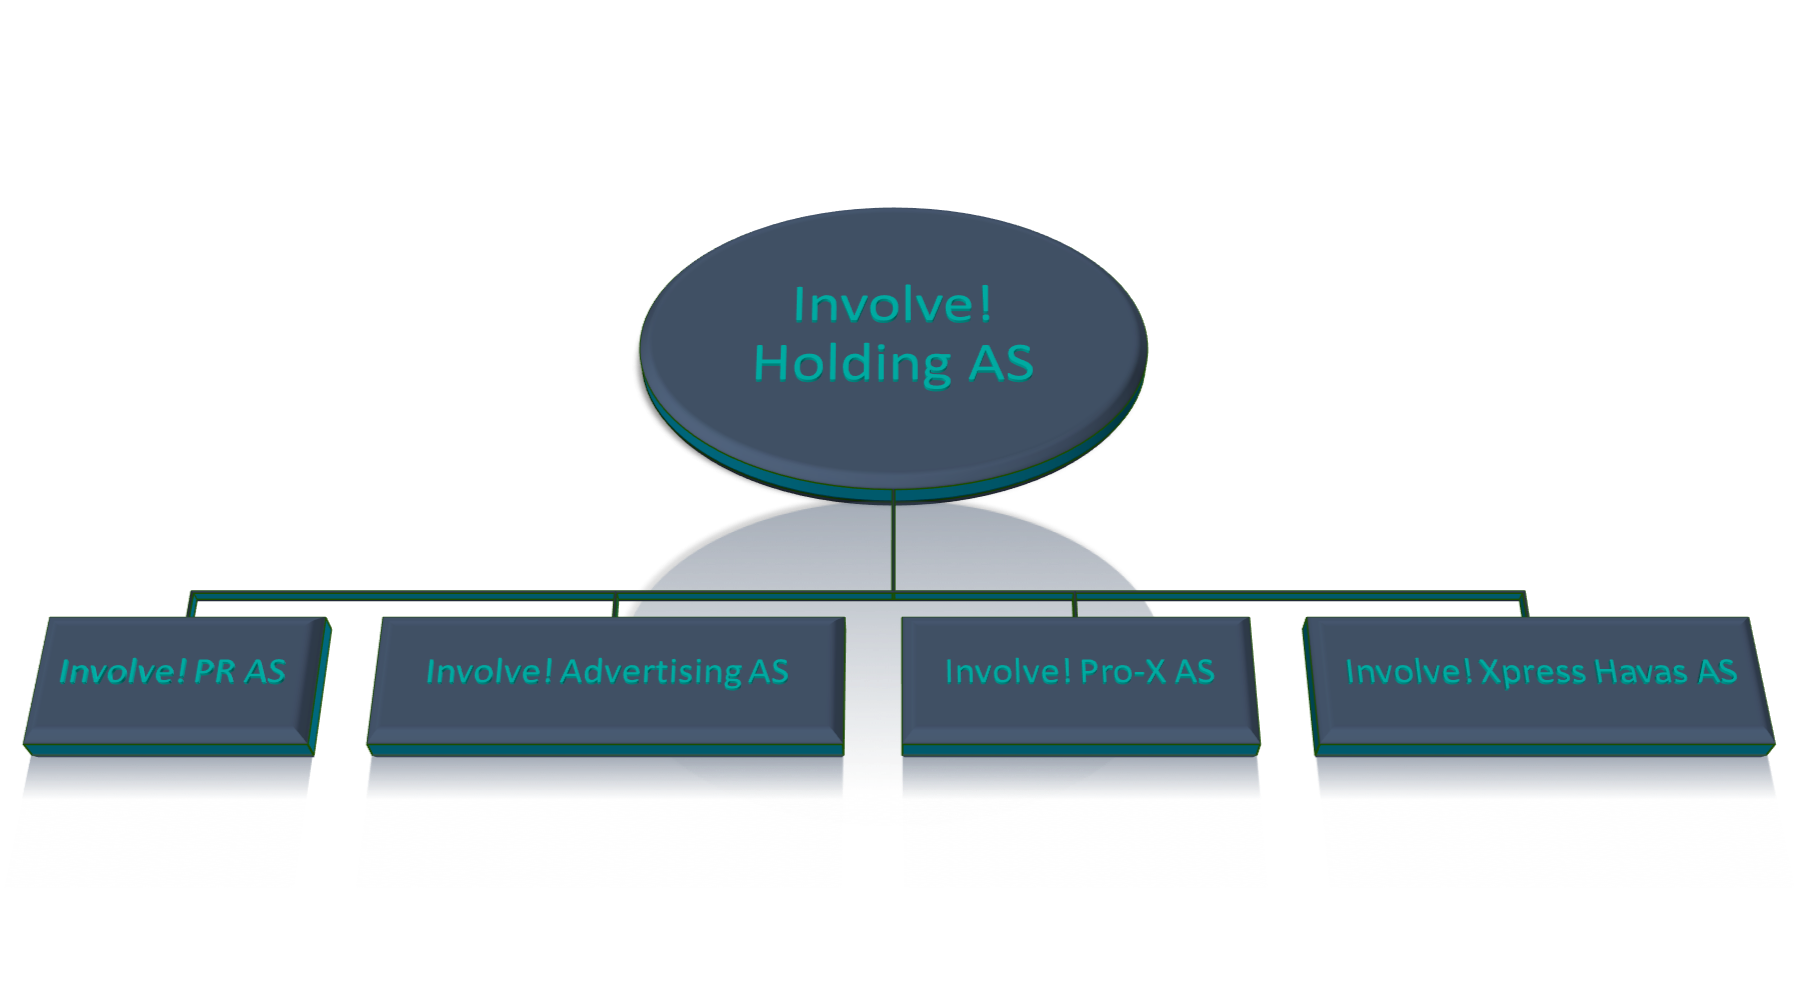
\includegraphics [scale=0.45]{bilder/org.png}
\caption{Organisasjonskart - Involve}
\label{fig:org}
\end{figure}

Kommunikasjonsbransjen er inne i en utvikling som kjennetegnes av økt digitalisering og en økning i tempo. Konkurransen blant aktørene anses som svært tøff, hvor oppdragene ofte blir lagt ut som åpne anbud. Prosjekter for kundene krever tverrfaglig kompetanse, og flere fagdisipliner må dermed samarbeide for å kunne levere et konkurransedyktig produkt. Dette fører til at det stilles sterkere krav til internkommunikasjonen enn tidligere.

\begin{figure}[H]
\centering
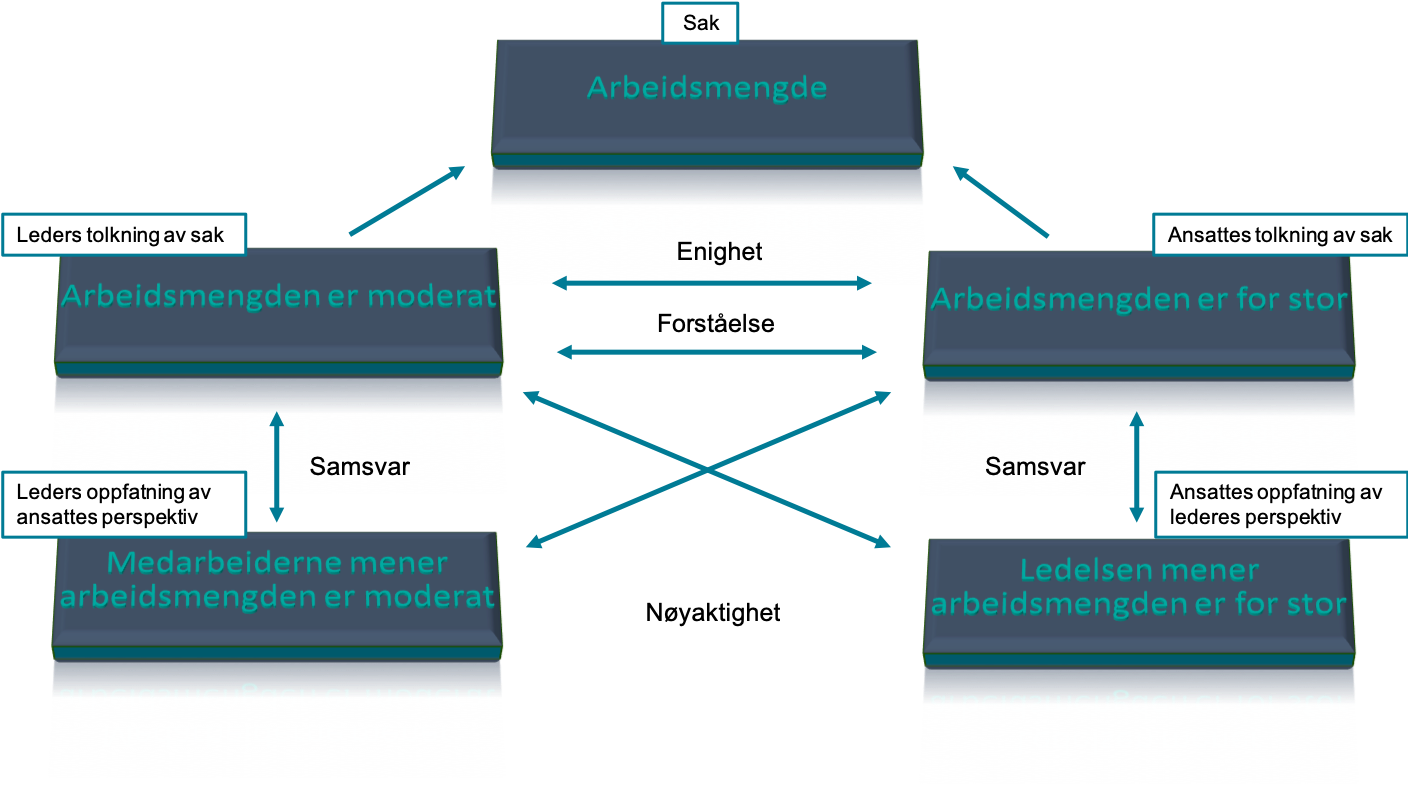
\includegraphics [scale=0.6]{bilder/koo.png}
\caption{Koorienteringsmodellen - arbeidsmengde}
\label{fig:koo}
\end{figure}
